%
% Einf�hrung in die Mustererkennung - WS2013
% Abgabeprotokoll Exercise 1
%
%

%{{{ misc
\documentclass[subfigure,epsfig,fleqn,float,numbers=noenddot]{scrartcl}

\usepackage{graphicx}
\usepackage{epstopdf}
\usepackage{caption}
\usepackage{subcaption}
\usepackage{amsmath}

\usepackage{pgfplots}

%Zitieren:
\usepackage[english]{babel}
%\usepackage[german]{babel}
\usepackage{babelbib} % f�r das Erstellen des Bibtex-Literaturverzeichnisses
\usepackage{cite}
%\selectbiblanguage{english}
%\selectbiblanguage{german}

%Peseudocode
\usepackage{algpseudocode}
\usepackage{algorithm}

%Fancy shit
\usepackage{url}

\usepackage[pdftitle={Computer Vision - 2nd Exercise Round},
 						pdfauthor={Matthias Gusenbauer},
						pdfauthor={Robin Mel�n},
						pdfauthor={David Pfahler},
            pdfsubject={Computer Vision},
            pdfborder={0 0 0}]{hyperref}


\usetikzlibrary{plotmarks}
\pgfplotsset{compat=newest} 
\pgfplotsset{plot coordinates/math parser=false}

%%%%%%%%%%%%%%%%%%%%%%%%%%%%%%%%
% Titlepage

\pagestyle{empty}


%set dimensions of columns, gap between columns, and paragraph indent

\setlength{\textheight}{24.7 cm}
\setlength{\columnsep}{1 cm}
\setlength{\textwidth}{16 cm}
%\setlength{\footheight}{0.0 cm}
\setlength{\topmargin}{0.0 cm}
\setlength{\headheight}{0.0 cm}
\setlength{\headsep}{-0.3 cm}
\setlength{\oddsidemargin}{0.0 cm}
\setlength{\parindent}{0 cm}
\setlength{\parskip}{0.5em}
\setlength{\mathindent}{0mm}

% set page counter if document is part of proceedings
\setcounter{page}{1}
\renewcommand{\floatpagefraction}{0.9}
\renewcommand{\textfraction}{0.1}

% Set the Counters like in the exercise sheet
\setcounter{section}{3}
\renewcommand{\thesection}{Assignment \arabic{section}:}
\renewcommand{\thesubsection}{\Alph{subsection}.}

%\renewcommand{\captionlabelfont}{\fontfamily{phv}\fontseries{bx}\fontsize{10}{10pt}\selectfont}
%\renewcommand{\captionfont}{\fontfamily{phv}\fontsize{10}{12pt}\selectfont}
%\setlength{\captionmargin}{0.5 cm}

\makeatletter
\makeatother
\def\RR{\hbox{I\kern-.2em\hbox{R}}}


\begin{document}

%don't want date printed
\date{\today}

%make title bold and 14 pt font (Latex default is non-bold, 16pt) 
\title{~\\
	\fontsize{12}{12pt} \bf Computer Vision 183.585 VU 3.0 4.5 ECTS
  ~\\[0.7cm]
  \fontsize{14}{14pt} \bf 2nd Exercise Round}
  

%for single author 
\author{~\\
  ~\\
  \fontsize{12}{12pt}
  {\bf David Pfahler, Matthias Gusenbauer, Robin Mel�n}\\
  1126287, 1125577, 1029201
  ~\\ ~\\ ~\\
  \normalsize
}

\maketitle
%I don't know why I have to reset thispagestyle, but otherwise get page numbers 
\normalfont
\thispagestyle{empty}

%%%%%%%%%%%%%%%%%%%%%%%%%%%%%%%%%%%%%%%%%%%%%%%%%%%%%%%%%%%%%%%%%%%%%%%%%%%%%%%%
% CONTENT

\section{Image Stitching}
\label{sec:1}

\subsection{SIFT Interest Point Detection}
\label{sec:A}

\subsection{Interest Point Matching and Image Registration}
\label{sec:B}

\subsection{Image Stitching}
\label{sec:C}

\section{Scene Recognition with Bag of VisualWords}
\label{sec:2}

\begin{figure}
		\centering
		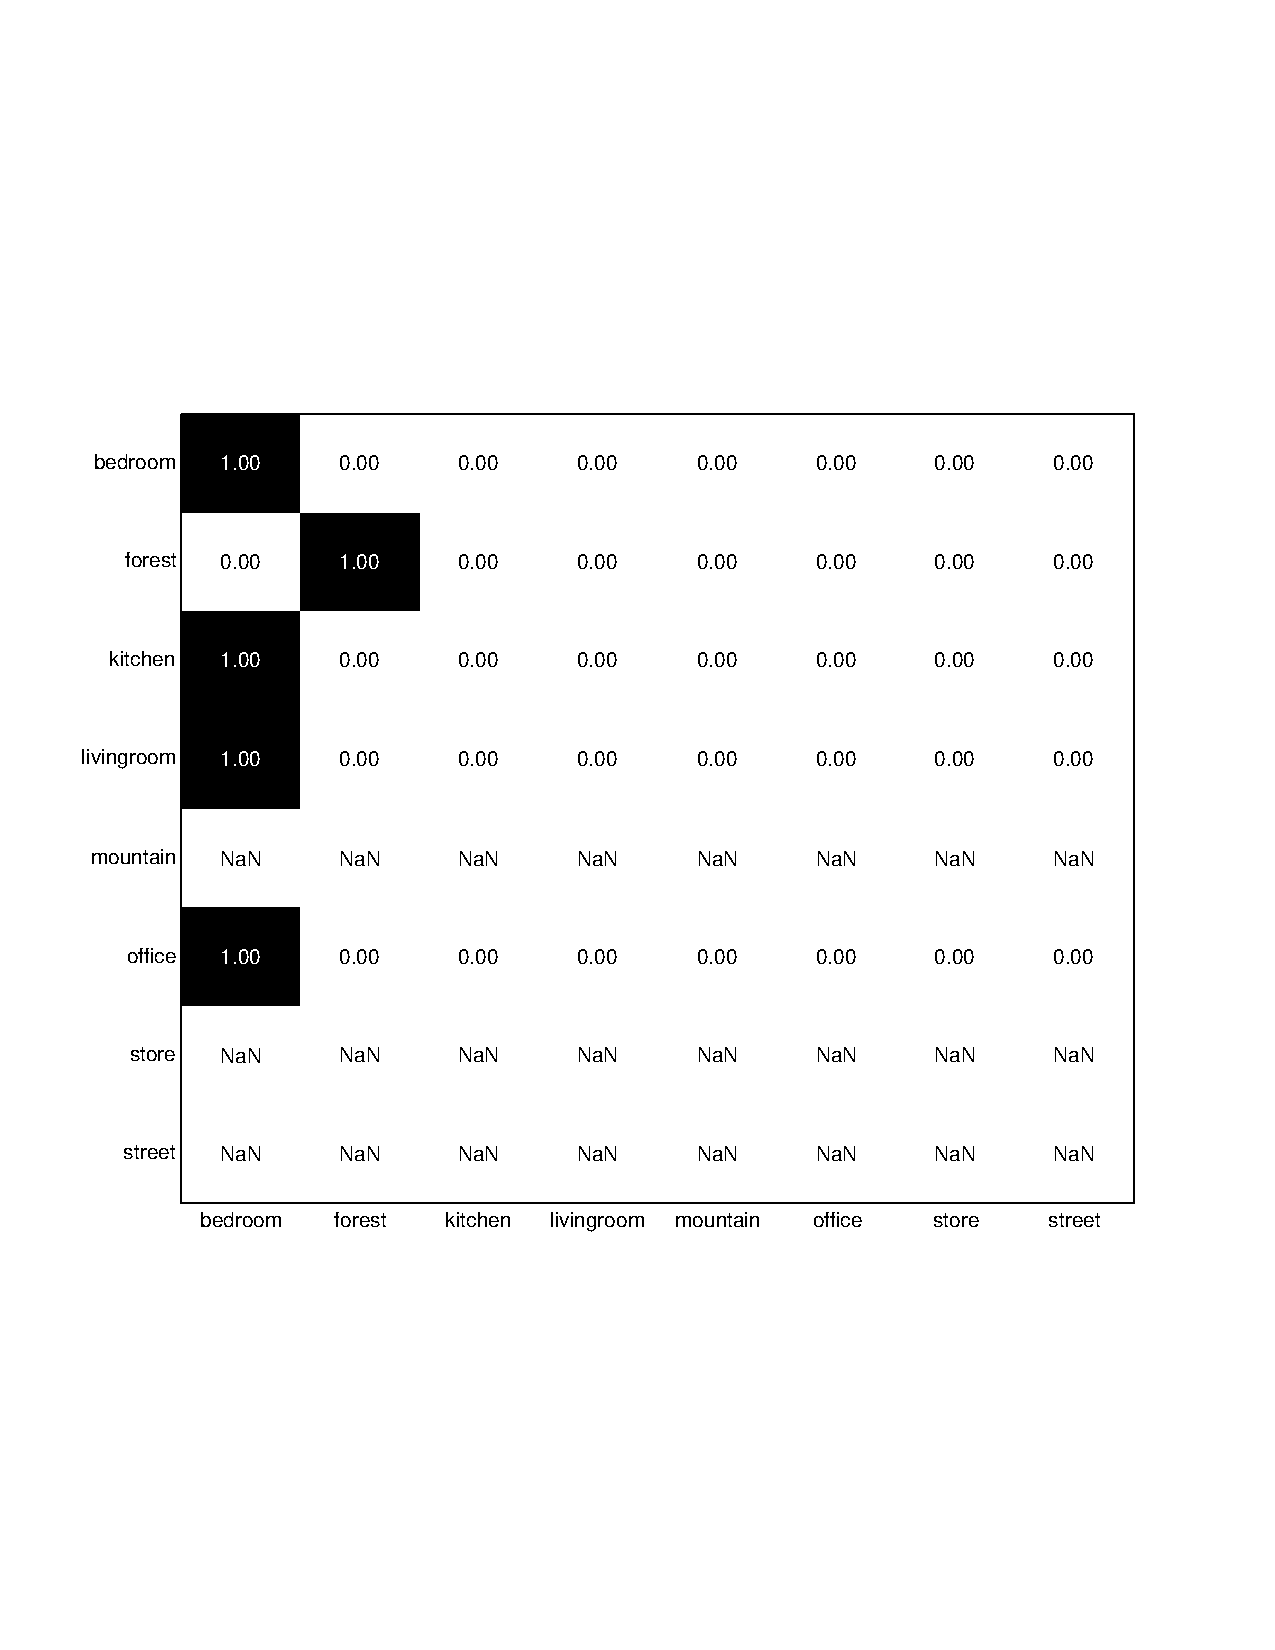
\includegraphics[width=\textwidth]{img/conf_matrix_own.pdf}
		\caption{Conf Matrix Own}
		\label{fig:conf_matrix_own}
\end{figure}
\begin{figure}
		\centering
		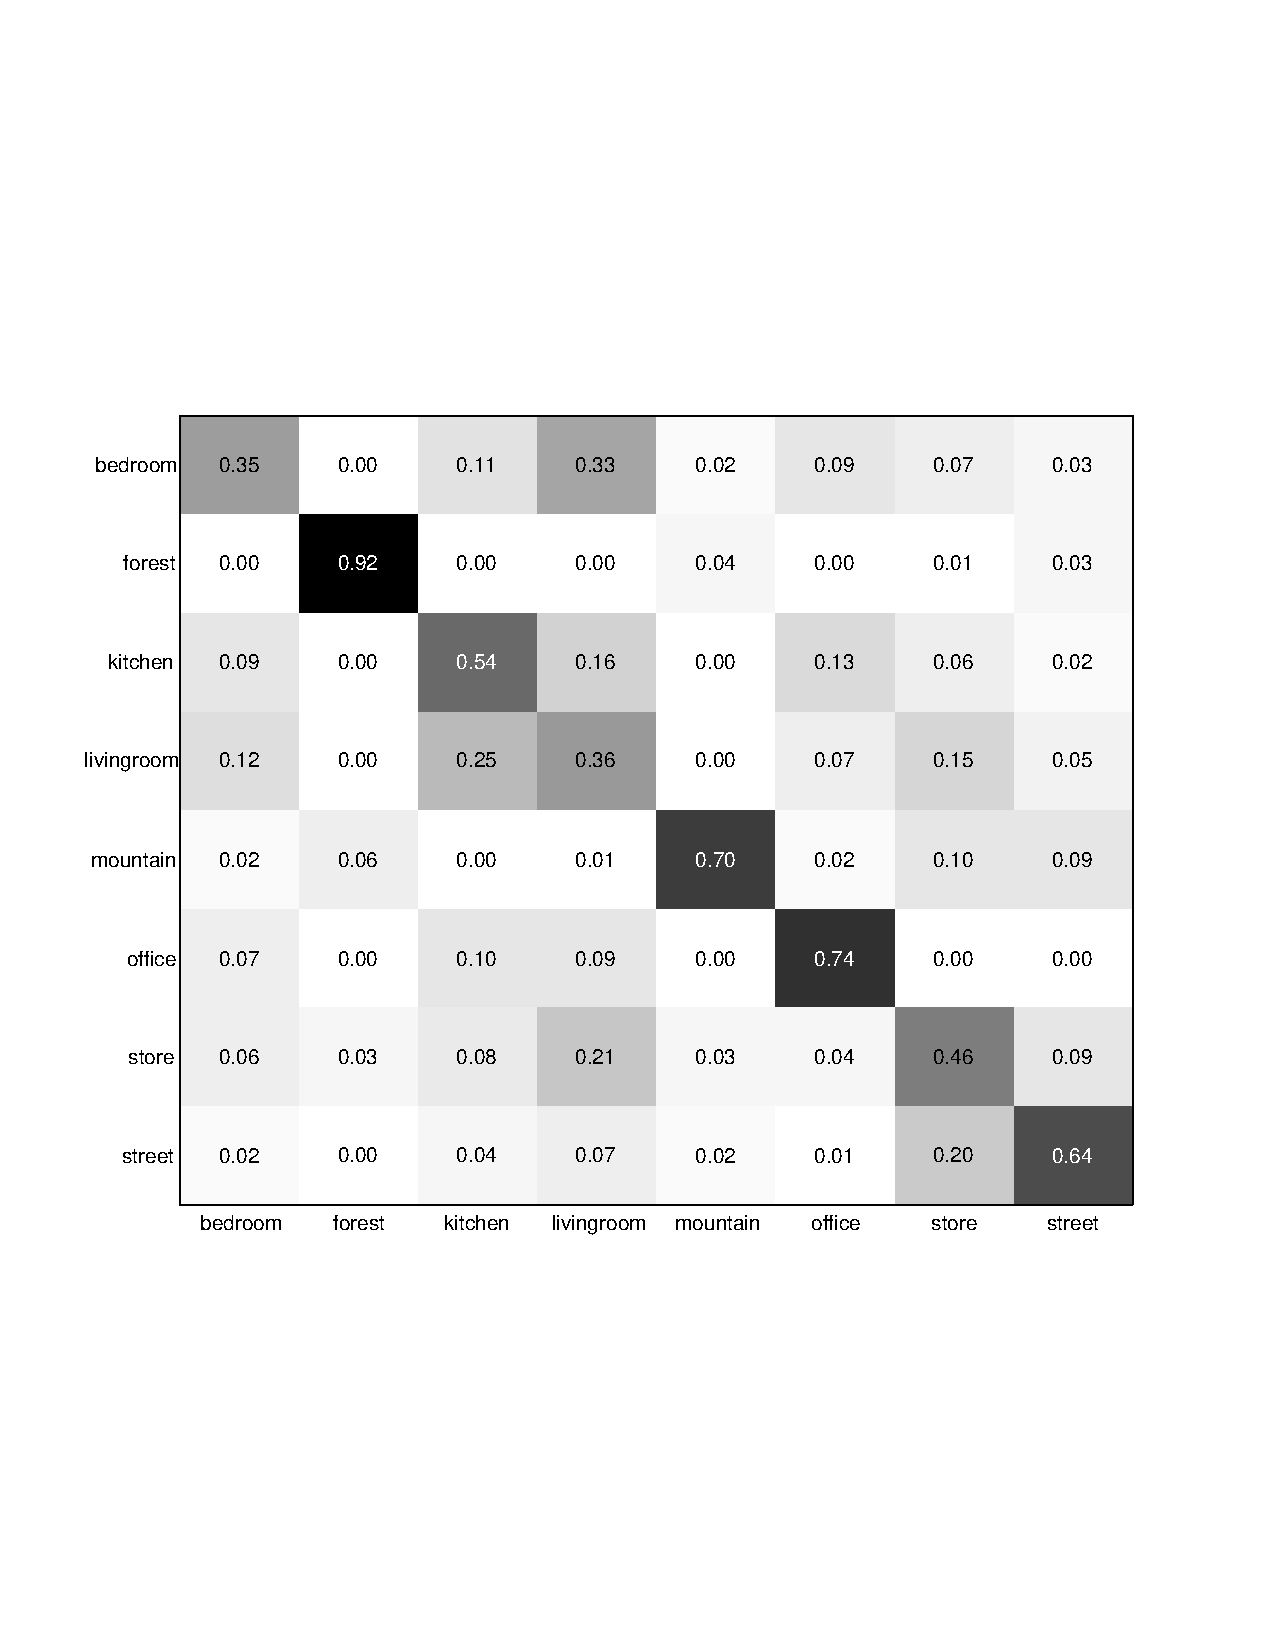
\includegraphics[width=\textwidth]{img/conf_matrix_test.pdf}
		\caption{Conf Matrix Test}
		\label{fig:conf_matrix_test}
\end{figure}

\end{document}

% vim:foldmethod=marker
